\documentclass[a4paper, UTF-8]{article}
\usepackage{algorithm}
\usepackage{algpseudocode}
\usepackage{amsmath}
\usepackage{amsfonts}
\usepackage{amsthm}
\usepackage{tikz}
\usetikzlibrary{automata, positioning, arrows}
\usepackage[utf8]{inputenc} % allow utf-8 input
\usepackage[T1]{fontenc}    % use 8-bit T1 fonts
\usepackage{hyperref}       % hyperlinks
\usepackage{url}            % simple URL typesetting
\usepackage{booktabs}       % professional-quality tables
\usepackage{amsfonts}       % blackboard math symbols
\usepackage{nicefrac}       % compact symbols for 1/2, etc.
\usepackage{microtype}      % microtypography
\usepackage{xcolor}         % colors

\theoremstyle{plain}
\newtheorem{theorem}{\indent Theorem}[section]
\newtheorem{lemma}[theorem]{\indent Lemma}
\newtheorem{assumption}{\indent Assumption}[section]
\newtheorem{note}[theorem]{\indent Notation}
\newtheorem{proposition}[theorem]{\indent Proposition}
\newtheorem{corollary}[theorem]{\indent Corollary}
\newtheorem{definition}{\indent Definition}[section]
\newtheorem{example}{\indent Example}[section]
\newtheorem{remark}{\indent Remark}[section]
\newenvironment{solution}{\begin{proof}[\indent\bf Solution]}{\end{proof}}
\renewcommand{\proofname}{\indent\bf Proof}

\begin{document}

\title{\bf{Lab3 Answers}}

\author{Yanqiao Chen*\\ 
  Department of Computer Science and Engineering\\
  Southern University of Science and Technology\\
  \texttt{12412115@mail.sustech.edu.cn}
  }

\maketitle

\section{Question 1}

\begin{itemize}
    \item [a.] $1\Sigma^*0$ 
    \item [b.] $\Sigma^*1\Sigma^*1\Sigma^*1 \Sigma^*$ 
    \item [c.] $\Sigma^*0101\Sigma^*$ 
    \item [d.] $\Sigma^2 0\Sigma^*$ 
    \item [e.] $(0(\Sigma^2)^*)\cup (1(\Sigma^2)^*\Sigma) $ 
    \item [f.] $(0 \cup 10)^* 1^*$
    \item [g.] $(\Sigma \cup \epsilon)^*$ 
    \item [h.] $\epsilon \cup 1 \cup 0\Sigma^* \cup 10\Sigma^* \cup 110\Sigma^* \cup 111\Sigma^+$
    \item [i.] $(1 \Sigma)^*(1 \cup \epsilon)$ 
    \item [j.] $000^* \cup 1000^* \cup 0100^* \cup 0010^* \cup 000^* 1 0^*$
    \item [k.] $\epsilon \cup 0$
    \item [l.] $(1 \cup 01^*0)^*\cup 0^*10^*10^*$
    \item [m.] $\emptyset$
    \item [n.] $\Sigma^+$
\end{itemize}

\section{Question 2} 

\subsection{a)} 

We draw the NFA as follows: 

\begin{center}
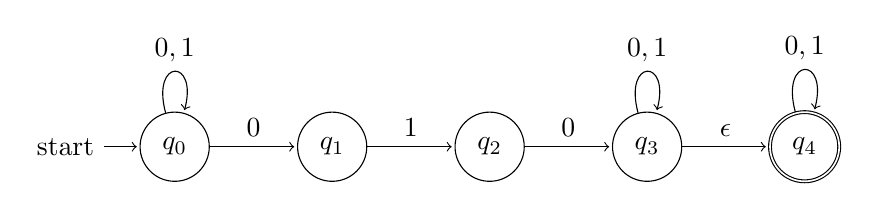
\begin{tikzpicture}[shorten >=1pt, node distance=2cm, on grid, auto]
    \node[state, initial] (q0) {$q_0$};
    \node[state, right=of q0] (q1) {$q_1$};
    \node[state, right=of q1] (q2) {$q_2$};
    \node[state, right=of q2] (q3) {$q_3$};
    \node[state, accepting, right=of q3] (q4) {$q_4$};
    
    \path[->]
        (q0) edge[loop above] node {$0, 1$} ()
        (q0) edge node {$0$} (q1)
        (q1) edge node {$1$} (q2)
        (q2) edge node {$0$} (q3)
        (q3) edge node {$\epsilon$} (q4)
        (q3) edge[loop above] node {$0, 1$} ()
        (q4) edge[loop above] node {$0, 1$} ();
\end{tikzpicture}
\end{center}

\subsection{b)}

For $(((11)^*(00)) \cup 01)^*$, we construct the NFA using Thompson's construction:

\begin{center}
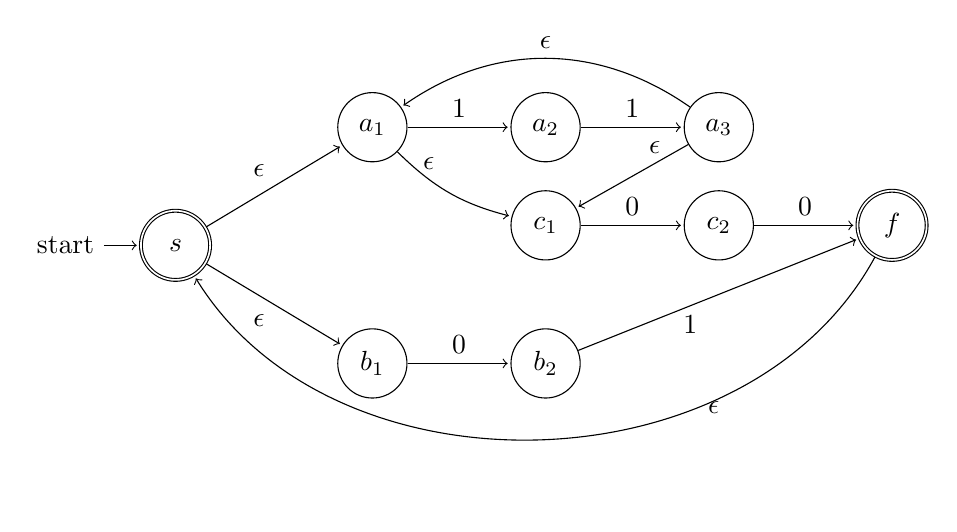
\begin{tikzpicture}[shorten >=1pt, node distance=2.2cm, on grid, auto]
    % Top branch states (11)*
    \node[state, initial, accepting] (s) {$s$};
    \node[state, above right=1.5cm and 2.5cm of s] (a1) {$a_1$};
    \node[state, right=of a1] (a2) {$a_2$};
    \node[state, right=of a2] (a3) {$a_3$};
    
    % Bottom branch states 01
    \node[state, below right=1.5cm and 2.5cm of s] (b1) {$b_1$};
    \node[state, right=of b1] (b2) {$b_2$};
    
    % (00) states - positioned to the right, aligned between top and bottom
    \node[state, right=3.5cm of a2, below=0.8cm] (c1) {$c_1$};
    \node[state, right=of c1] (c2) {$c_2$};
    \node[state, accepting, right=of c2] (f) {$f$};
    
    \path[->]
        % Entry to two branches
        (s) edge node[above left] {$\epsilon$} (a1)
        (s) edge node[below left] {$\epsilon$} (b1)
        
        % Branch 1: (11)*
        (a1) edge node {$1$} (a2)
        (a2) edge node {$1$} (a3)
        (a3) edge[bend right=35] node[above] {$\epsilon$} (a1)
        
        % From (11)* to (00)
        (a1) edge[bend right=15] node[above, pos=0.3] {$\epsilon$} (c1)
        (a3) edge node[above, pos=0.3] {$\epsilon$} (c1)
        
        % (00) part
        (c1) edge node {$0$} (c2)
        (c2) edge node {$0$} (f)
        
        % Branch 2: 01
        (b1) edge node {$0$} (b2)
        (b2) edge node[below, pos=0.4] {$1$} (f)
        
        % Loop back for Kleene star
        (f) edge[bend left=60] node[right, pos=0.3] {$\epsilon$} (s);
\end{tikzpicture}
\end{center}

\textbf{Explanation:} This NFA uses Thompson's construction:
- Start state $s$ is also accepting (for $\epsilon$ in the outer $^*$)
- Top branch: $(11)^*$ followed by $(00)$ - matches even number of 1s followed by 00
- Bottom branch: $01$ - matches 01
- After either branch completes, we can loop back to $s$ for the outer Kleene star

\subsection{c)}

\begin{center}
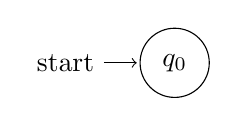
\begin{tikzpicture}[shorten >=1pt, node distance=2cm, on grid, auto]
    \node[state, initial] (q0) {$q_0$};
\end{tikzpicture}
\end{center}

\section{Question 3} 

For the DFA in Question 3(a), we convert it to a regular expression using the state elimination method.

\subsection{Step 1: Original NFA (Figure a)}

Original NFA with states 1 (initial) and 2 (accepting):

\begin{center}
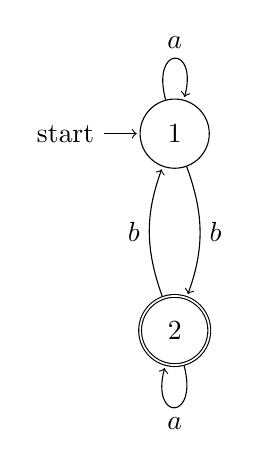
\begin{tikzpicture}[shorten >=1pt, node distance=2.5cm, on grid, auto]
    \node[state, initial] (q1) {$1$};
    \node[state, accepting, below=of q1] (q2) {$2$};
    
    \path[->]
        (q1) edge[loop above] node {$a$} ()
        (q1) edge[bend left=20] node {$b$} (q2)
        (q2) edge[bend left=20] node {$b$} (q1)
        (q2) edge[loop below] node {$a$} ();
\end{tikzpicture}
\end{center}

\subsection{Step 2: Add New Start and Accept States}

We add a new start state $s$ and a new accept state $f$ with $\epsilon$-transitions:

\begin{center}
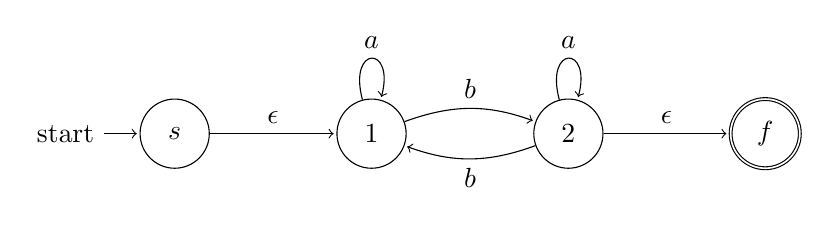
\begin{tikzpicture}[shorten >=1pt, node distance=2.5cm, on grid, auto]
    \node[state, initial] (s) {$s$};
    \node[state, right=of s] (q1) {$1$};
    \node[state, right=of q1] (q2) {$2$};
    \node[state, accepting, right=of q2] (f) {$f$};
    
    \path[->]
        (s) edge node {$\epsilon$} (q1)
        (q1) edge[loop above] node {$a$} ()
        (q1) edge[bend left=20] node {$b$} (q2)
        (q2) edge[bend left=20] node {$b$} (q1)
        (q2) edge[loop above] node {$a$} ()
        (q2) edge node {$\epsilon$} (f);
\end{tikzpicture}
\end{center}

\subsection{Step 3: Eliminate State 2}

When eliminating state 2, we need to consider:
\begin{itemize}
    \item Path $1 \to 2 \to f$: label is $b \cdot a^* \cdot \epsilon = ba^*$
    \item Path $1 \to 2 \to 1$: label is $b \cdot a^* \cdot b = ba^*b$
\end{itemize}

After eliminating state 2:

\begin{center}
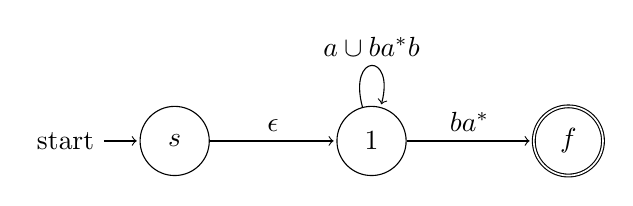
\begin{tikzpicture}[shorten >=1pt, node distance=2.5cm, on grid, auto]
    \node[state, initial] (s) {$s$};
    \node[state, right=of s] (q1) {$1$};
    \node[state, accepting, right=of q1] (f) {$f$};
    
    \path[->]
        (s) edge node {$\epsilon$} (q1)
        (q1) edge[loop above] node {$a \cup ba^*b$} ()
        (q1) edge node {$ba^*$} (f);
\end{tikzpicture}
\end{center}

\subsection{Step 4: Eliminate State 1}

After eliminating state 1, the regular expression on the edge from $s$ to $f$ is:

\begin{center}
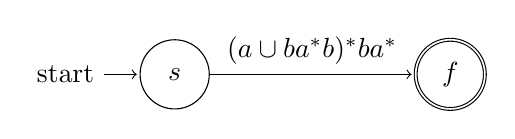
\begin{tikzpicture}[shorten >=1pt, node distance=3.5cm, on grid, auto]
    \node[state, initial] (s) {$s$};
    \node[state, accepting, right=of s] (f) {$f$};
    
    \path[->]
        (s) edge node {$(a \cup ba^*b)^*ba^*$} (f);
\end{tikzpicture}
\end{center}

\textbf{Final Answer:} The regular expression for the NFA in 3(a) is:
\[
\boxed{(a \cup ba^*b)^*ba^*}
\]

\subsection{Question 3(b)}

For the DFA in Question 3(b), states 1 and 3 are accepting. We follow the same procedure.

\textbf{Step 1:} Add new start state $s$ and new accept state $f$:

\begin{center}
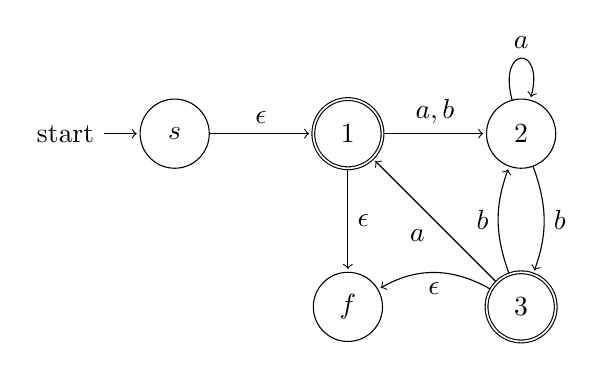
\begin{tikzpicture}[shorten >=1pt, node distance=2.2cm, on grid, auto]
    \node[state, initial] (s) {$s$};
    \node[state, right=of s, accepting] (q1) {$1$};
    \node[state, right=of q1] (q2) {$2$};
    \node[state, below=of q2, accepting] (q3) {$3$};
    \node[state, below=of q1] (f) {$f$};
    
    \path[->]
        (s) edge node {$\epsilon$} (q1)
        (q1) edge node {$a,b$} (q2)
        (q1) edge node {$\epsilon$} (f)
        (q2) edge[loop above] node {$a$} ()
        (q2) edge[bend left=20] node {$b$} (q3)
        (q3) edge[bend left=20] node {$b$} (q2)
        (q3) edge node {$a$} (q1)
        (q3) edge[bend right=30] node[below] {$\epsilon$} (f);
\end{tikzpicture}
\end{center}

\textbf{Step 2:} Eliminate state 2:

State 2 has self-loop $a$ and transitions to/from state 3 with $b$. When eliminated:
\begin{itemize}
    \item $1 \to 3$ via 2: $(a \cup b) \cdot a^* \cdot b$
    \item $3 \to 3$ via 2: $b \cdot a^* \cdot b$
\end{itemize}

\begin{center}
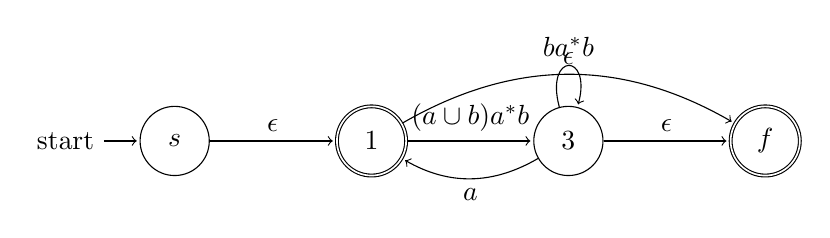
\begin{tikzpicture}[shorten >=1pt, node distance=2.5cm, on grid, auto]
    \node[state, initial] (s) {$s$};
    \node[state, right=of s, accepting] (q1) {$1$};
    \node[state, right=of q1] (q3) {$3$};
    \node[state, accepting, right=of q3] (f) {$f$};
    
    \path[->]
        (s) edge node {$\epsilon$} (q1)
        (q1) edge node {$(a \cup b)a^*b$} (q3)
        (q1) edge[bend left=30] node[above] {$\epsilon$} (f)
        (q3) edge[bend left=30] node[below] {$a$} (q1)
        (q3) edge[loop above] node {$ba^*b$} ()
        (q3) edge node {$\epsilon$} (f);
\end{tikzpicture}
\end{center}

\textbf{Step 3:} Eliminate state 3:

We have paths involving state 3. The self-loop on 3 is $(ba^*b)^*$, and we need to compute the new edges:
\begin{itemize}
    \item From 1 to 1 via 3: $(a \cup b)a^*b(ba^*b)^*a$
    \item From 1 to f via 3: $(a \cup b)a^*b(ba^*b)^*$
\end{itemize}

After eliminating state 3:

\begin{center}
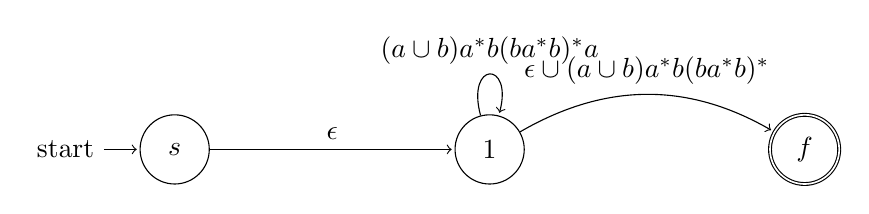
\begin{tikzpicture}[shorten >=1pt, node distance=4cm, on grid, auto]
    \node[state, initial] (s) {$s$};
    \node[state, right=of s] (q1) {$1$};
    \node[state, accepting, right=of q1] (f) {$f$};
    
    \path[->]
        (s) edge node {$\epsilon$} (q1)
        (q1) edge[loop above] node {$(a \cup b)a^*b(ba^*b)^*a$} ()
        (q1) edge[bend left=30] node[above] {$\epsilon \cup (a \cup b)a^*b(ba^*b)^*$} (f);
\end{tikzpicture}
\end{center}

\textbf{Step 4:} Eliminate state 1 to get the final regular expression:

\begin{center}
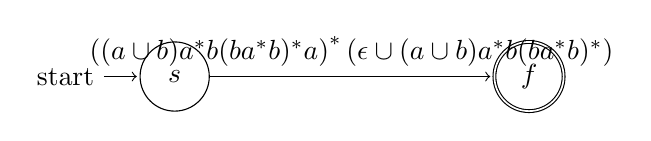
\begin{tikzpicture}[shorten >=1pt, node distance=4.5cm, on grid, auto]
    \node[state, initial] (s) {$s$};
    \node[state, accepting, right=of s] (f) {$f$};
    
    \path[->]
        (s) edge node {$\left((a \cup b)a^*b(ba^*b)^*a\right)^*\left(\epsilon \cup (a \cup b)a^*b(ba^*b)^*\right)$} (f);
\end{tikzpicture}
\end{center}

\textbf{Final Answer for 3(b):}
\[
\boxed{\left((a + b)a^*b(ba^*b)^*a\right)^*\left(\epsilon \cup (a + b)a^*b(ba^*b)^*\right)}
\]


\section{Question 4}

Language $C$: strings beginning with `/\#`, ending with `\#/`, with \textbf{no intervening `\#/`} in between.

\subsection{a) DFA for Comment Language $C$}

The key constraint is that inside the comment body, we cannot have the substring `\#/`. This means after seeing `\#`, if the next character is `/`, we must end the comment. But if it's `a`, `b`, or another `\#`, we continue.

\begin{center}
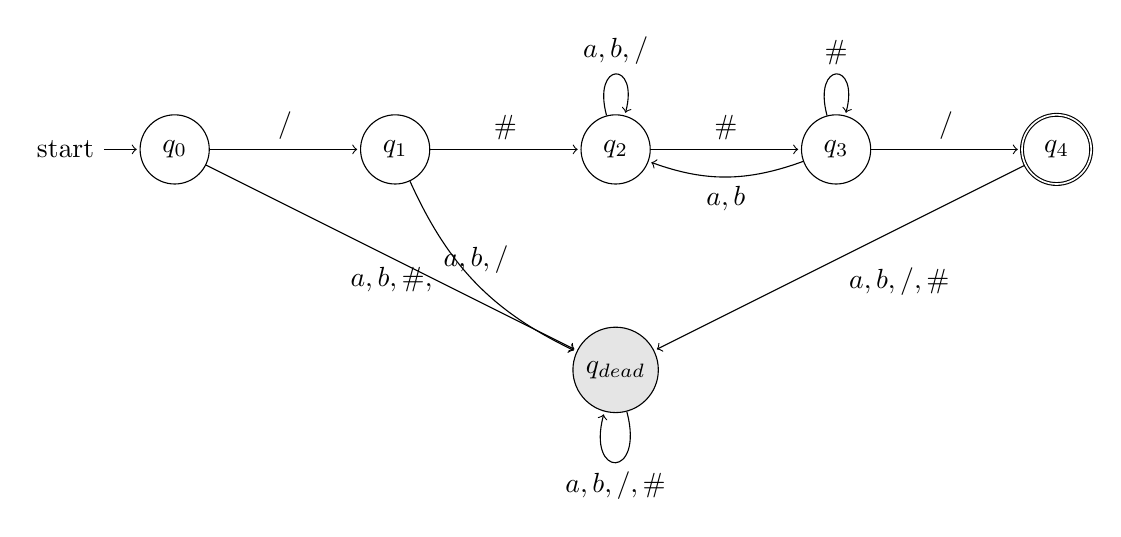
\begin{tikzpicture}[shorten >=1pt, node distance=2.8cm, on grid, auto]
    % States
    \node[state, initial] (q0) {$q_0$};
    \node[state, right=of q0] (q1) {$q_1$};
    \node[state, right=of q1] (q2) {$q_2$};
    \node[state, right=of q2] (q3) {$q_3$};
    \node[state, accepting, right=of q3] (q4) {$q_4$};
    \node[state, below=of q2, fill=gray!20] (dead) {$q_{dead}$};
    
    % Transitions
    \path[->]
        % q0: waiting for /
        (q0) edge node {$/$} (q1)
        (q0) edge node[below] {$a,b,\#,$} (dead)
        
        % q1: saw /, waiting for #
        (q1) edge node {$\#$} (q2)
        (q1) edge[bend right=20] node[above] {$a,b,/$} (dead)
        
        % q2: inside comment body (saw /#), can read a, b, / freely
        (q2) edge[loop above] node {$a,b,/$} ()
        (q2) edge node {$\#$} (q3)
        
        % q3: saw # inside comment, waiting for / to end
        (q3) edge node {$/$} (q4)
        (q3) edge[loop above] node {$\#$} ()
        (q3) edge[bend left=20] node {$a,b$} (q2)
        
        % q4: accepting state (comment properly closed)
        (q4) edge node {$a,b,/,\#$} (dead);
    
    % Dead state self-loop
    \path[->] (dead) edge[loop below] node {$a,b,/,\#$} ();
\end{tikzpicture}
\end{center}

\subsection{b) Regular Expression for $C$ via State Elimination}

We first construct an NFA, then apply state elimination.

\textbf{Step 1: NFA Construction}

The NFA uses Thompson's construction with special handling to prevent `\#/` inside the comment body:

\begin{center}
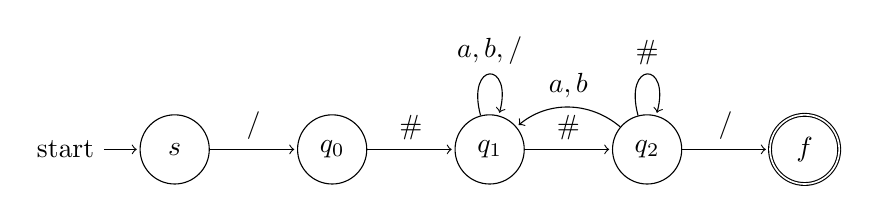
\begin{tikzpicture}[shorten >=1pt, node distance=2cm, on grid, auto]
    \node[state, initial] (s) {$s$};
    \node[state, right=of s] (q0) {$q_0$};
    \node[state, right=of q0] (q1) {$q_1$};
    \node[state, right=of q1] (q2) {$q_2$};
    \node[state, accepting, right=of q2] (f) {$f$};
    
    \path[->]
        % Recognize /#
        (s) edge node {$/$} (q0)
        (q0) edge node {$\#$} (q1)
        % Comment body: a, b, / (but not # followed by /)
        (q1) edge[loop above] node {$a,b,/$} ()
        (q1) edge node {$\#$} (q2)
        % After #: must see / to end, or go back if a, b, or another #
        (q2) edge node {$/$} (f)
        (q2) edge[loop above] node {$\#$} ()
        (q2) edge[bend right=40] node[above] {$a,b$} (q1);
\end{tikzpicture}
\end{center}

\textbf{Step 2: Add New Start and Accept States}

Convert to GNFA with new start $s'$ and accept $f'$:

\begin{center}
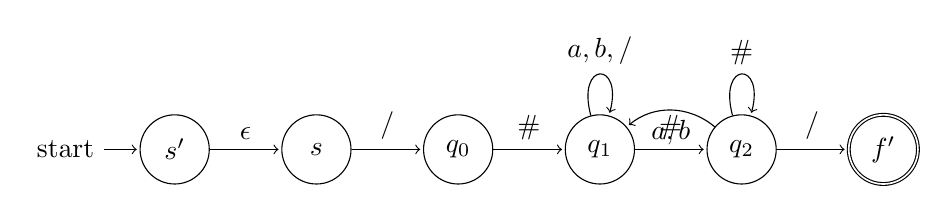
\begin{tikzpicture}[shorten >=1pt, node distance=1.8cm, on grid, auto]
    \node[state, initial] (sp) {$s'$};
    \node[state, right=of sp] (s) {$s$};
    \node[state, right=of s] (q0) {$q_0$};
    \node[state, right=of q0] (q1) {$q_1$};
    \node[state, right=of q1] (q2) {$q_2$};
    \node[state, accepting, right=of q2] (fp) {$f'$};
    
    \path[->]
        (sp) edge node {$\epsilon$} (s)
        (s) edge node {$/$} (q0)
        (q0) edge node {$\#$} (q1)
        (q1) edge[loop above] node {$a,b,/$} ()
        (q1) edge node {$\#$} (q2)
        (q2) edge node {$/$} (fp)
        (q2) edge[loop above] node {$\#$} ()
        (q2) edge[bend right=40] node[below] {$a,b$} (q1);
\end{tikzpicture}
\end{center}

\textbf{Step 3: Eliminate State $s$}

\begin{center}
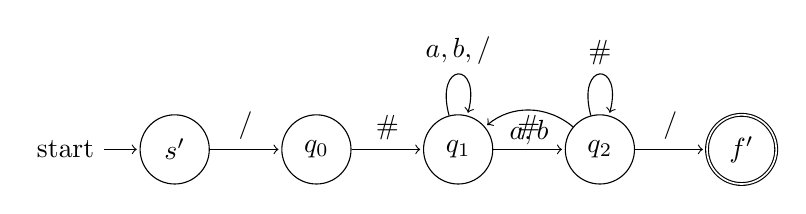
\begin{tikzpicture}[shorten >=1pt, node distance=1.8cm, on grid, auto]
    \node[state, initial] (sp) {$s'$};
    \node[state, right=of sp] (q0) {$q_0$};
    \node[state, right=of q0] (q1) {$q_1$};
    \node[state, right=of q1] (q2) {$q_2$};
    \node[state, accepting, right=of q2] (fp) {$f'$};
    
    \path[->]
        (sp) edge node {$/$} (q0)
        (q0) edge node {$\#$} (q1)
        (q1) edge[loop above] node {$a,b,/$} ()
        (q1) edge node {$\#$} (q2)
        (q2) edge node {$/$} (fp)
        (q2) edge[loop above] node {$\#$} ()
        (q2) edge[bend right=40] node[below] {$a,b$} (q1);
\end{tikzpicture}
\end{center}

\textbf{Step 4: Eliminate State $q_0$}

\begin{center}
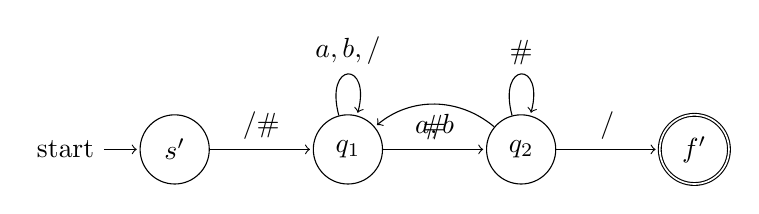
\begin{tikzpicture}[shorten >=1pt, node distance=2.2cm, on grid, auto]
    \node[state, initial] (sp) {$s'$};
    \node[state, right=of sp] (q1) {$q_1$};
    \node[state, right=of q1] (q2) {$q_2$};
    \node[state, accepting, right=of q2] (fp) {$f'$};
    
    \path[->]
        (sp) edge node {$/\#$} (q1)
        (q1) edge[loop above] node {$a,b,/$} ()
        (q1) edge node {$\#$} (q2)
        (q2) edge node {$/$} (fp)
        (q2) edge[loop above] node {$\#$} ()
        (q2) edge[bend right=40] node[below] {$a,b$} (q1);
\end{tikzpicture}
\end{center}

\textbf{Step 5: Eliminate State $q_2$}

State $q_2$ has:
- Self-loop: $\#$
- To $f'$: $/$
- To $q_1$: $a \cup b$

When eliminating $q_2$:
- New edge $q_1 \to f'$: $\# \cdot \#^* \cdot / = \#^+/$
- New self-loop on $q_1$: $\# \cdot \#^* \cdot (a \cup b) = \#^+(a \cup b)$

\begin{center}
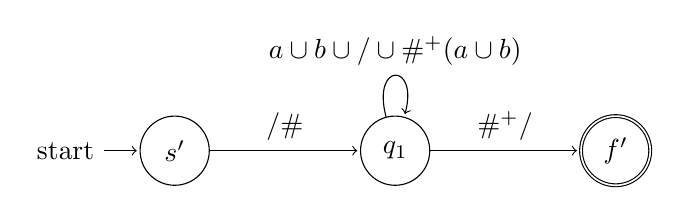
\begin{tikzpicture}[shorten >=1pt, node distance=2.8cm, on grid, auto]
    \node[state, initial] (sp) {$s'$};
    \node[state, right=of sp] (q1) {$q_1$};
    \node[state, accepting, right=of q1] (fp) {$f'$};
    
    \path[->]
        (sp) edge node {$/\#$} (q1)
        (q1) edge[loop above] node {$a \cup b \cup / \cup \#^+(a \cup b)$} ()
        (q1) edge node {$\#^+/$} (fp);
\end{tikzpicture}
\end{center}

Simplifying the self-loop on $q_1$:
\[
a \cup b \cup / \cup \#^+(a \cup b) = (a \cup b)(\epsilon \cup \#^+) \cup / = \#^*(a \cup b) \cup /
\]

\textbf{Step 6: Eliminate State $q_1$}

\begin{center}
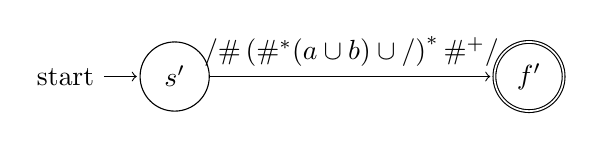
\begin{tikzpicture}[shorten >=1pt, node distance=4.5cm, on grid, auto]
    \node[state, initial] (sp) {$s'$};
    \node[state, accepting, right=of sp] (fp) {$f'$};
    
    \path[->]
        (sp) edge node {$/\#\left(\#^*(a \cup b) \cup /\right)^*\#^+/$} (fp);
\end{tikzpicture}
\end{center}

\textbf{Final Answer:}
\[
\boxed{/\#\left(\#^*(a \cup b) \cup /\right)^*\#^+/}
\]

\section{Question 5}

\begin{proof}
Let $R$ be a regular expression for $A$. We prove by \textbf{structural induction} on $R$ that there exists a regular expression $R^{\mathcal{R}}$ such that $L(R^{\mathcal{R}}) = L(R)^{\mathcal{R}}$.

\textbf{Base Cases:}
\begin{itemize}
    \item $R = \emptyset$: Define $\emptyset^{\mathcal{R}} = \emptyset$. Then $L(\emptyset^{\mathcal{R}}) = \emptyset = \emptyset^{\mathcal{R}}$.
    \item $R = \varepsilon$: Define $\varepsilon^{\mathcal{R}} = \varepsilon$. Then $L(\varepsilon^{\mathcal{R}}) = \{\varepsilon\} = \{\varepsilon\}^{\mathcal{R}}$.
    \item $R = a$ for $a \in \Sigma$: Define $a^{\mathcal{R}} = a$. Then $L(a^{\mathcal{R}}) = \{a\} = \{a\}^{\mathcal{R}}$.
\end{itemize}

\textbf{Inductive Steps:} Assume $R_1$ and $R_2$ are regular expressions with $L(R_1^{\mathcal{R}}) = L(R_1)^{\mathcal{R}}$ and $L(R_2^{\mathcal{R}}) = L(R_2)^{\mathcal{R}}$.

\begin{itemize}
    \item \textbf{Union:} $R = R_1 \cup R_2$. Define $(R_1 \cup R_2)^{\mathcal{R}} = R_1^{\mathcal{R}} \cup R_2^{\mathcal{R}}$.
    
    \item \textbf{Concatenation:} $R = R_1 R_2$. Define $(R_1 R_2)^{\mathcal{R}} = R_2^{\mathcal{R}} R_1^{\mathcal{R}}$.
    
    \item \textbf{Kleene Star:} $R = R_1^*$. Define $(R_1^*)^{\mathcal{R}} = (R_1^{\mathcal{R}})^*$.
\end{itemize}

By structural induction, for any regular expression $R$, there exists $R^{\mathcal{R}}$ with $L(R^{\mathcal{R}}) = L(R)^{\mathcal{R}}$. Therefore, if $A$ is regular, so is $A^{\mathcal{R}}$.
\end{proof}

\section{Question 6} 

\begin{proof}
We construct a DFA $M = (Q, \Sigma, \delta, q_0, F)$ with $n$ states that recognizes $B_n$:

\begin{itemize}
    \item $Q = \{q_0, q_1, \ldots, q_{n-1}\}$ (track the count of $a$'s modulo $n$)
    \item $\Sigma = \{a\}$
    \item $\delta(q_i, a) = q_{(i+1) \bmod n}$ for $0 \leq i < n$
    \item $q_0$ is the initial state
    \item $F = \{q_0\}$ (accept when the count is divisible by $n$)
\end{itemize}

\begin{center}
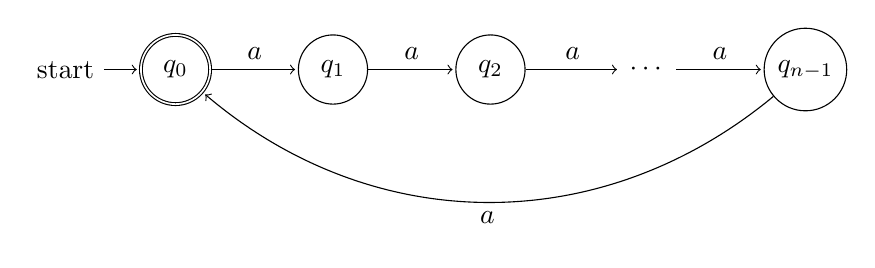
\begin{tikzpicture}[shorten >=1pt, node distance=2cm, on grid, auto]
    \node[state, initial, accepting] (q0) {$q_0$};
    \node[state, right=of q0] (q1) {$q_1$};
    \node[state, right=of q1] (q2) {$q_2$};
    \node[right=of q2] (dots) {$\cdots$};
    \node[state, right=of dots] (qn-1) {$q_{n-1}$};
    
    \path[->]
        (q0) edge node {$a$} (q1)
        (q1) edge node {$a$} (q2)
        (q2) edge node {$a$} (dots)
        (dots) edge node {$a$} (qn-1)
        (qn-1) edge[bend left=40] node[below] {$a$} (q0);
\end{tikzpicture}
\end{center}

This DFA accepts exactly $B_n = \{a^{pn} \mid p \geq 0\}$ since it returns to the accepting state $q_0$ after reading every $n$ consecutive $a$'s. Therefore, $B_n$ is regular.
\end{proof}

\end{document}
